\documentclass{article}

%% PACKAGES

% Fancy chapters with toc
\usepackage{titlesec,titletoc}

\usepackage[style=alphabetic, maxnames=4]{biblatex}
\addbibresource{references.bib}

\usepackage{amsmath,amsfonts,amsthm,amssymb,mathtools}
\usepackage[shortlabels]{enumitem}
\usepackage{imakeidx}
\makeindex[intoc] % Add index to bibliography.
\usepackage[bookmarksdepth=2]{hyperref}
\usepackage{xcolor}
\hypersetup{
	colorlinks=true,
	linkcolor={red!50!black},
	citecolor={blue!50!black},
	urlcolor={blue!80!black}
}
\usepackage{cleveref}
\usepackage{tikz-cd}
\usepackage{aligned-overset}
\usepackage{tcolorbox}
\tcbuselibrary{breakable}
% \tcbuselibrary{theorems}
\tcbuselibrary{skins}
\usepackage{microtype}
\usepackage{nicematrix}
\NiceMatrixOptions{cell-space-limits = 5pt}

\renewcommand{\thechapter}{\Roman{chapter}}
\counterwithout{section}{chapter}
\counterwithout{figure}{chapter}
\counterwithout{table}{chapter}
\renewcommand*\thesection{\arabic{section}}

\titleformat{\chapter}[display]
{\bfseries\Large}
{\filleft
	\MakeUppercase{\chaptertitlename} \Huge\thechapter}
{3ex}
{\titlerule
	\vspace{2ex}%
	\filright}
[{%
			\vspace{2ex}%
			\titlerule
		}]

\titlecontents{chapter}
[0pt]
{\addvspace{1pc}}%
{\contentsmargin{0pt}%
	\bfseries
	\makebox[0pt][r]{\huge\thecontentslabel\enspace}%
	\large}
{% \addvspace{.2pc}%
	\contentsmargin{0pt}%
	\large}
{}
[\addvspace{.5pc}]

\newcommand{\chaptertoc}{%
	\dotfill
	\vspace*{1ex}
	\startcontents[chapters]
	\printcontents[chapters]{}{1}[2]{}
	\vspace*{1ex}
	\noindent\dotfill\\
	\vspace*{1pc}
}
% \usepackage{fancyhdr}
% \pagestyle{fancy}

\usetikzlibrary{positioning,quotes,calc,patterns}

%% Equation numbered by section
\numberwithin{equation}{section}

%% Theorem environments
\theoremstyle{plain}
\newtheorem{theorem}{Theorem}[section]
\newtheorem{lemma}[theorem]{Lemma}
\newtheorem{proposition}[theorem]{Proposition}
\newtheorem{corollary}[theorem]{Corollary}

\newtheorem{condition}{Condition}
\renewcommand*{\thecondition}{\Alph{condition}}
\crefname{condition}{condition}{conditions}

\newtheorem*{convention}{Convention}
\newtheorem*{theorem*}{Theorem}
\newtheorem*{lemma*}{Lemma}
\newtheorem*{prop*}{Proposition}
\newtheorem*{corollary*}{Corollary}

\theoremstyle{definition}
\newtheorem{definition}[theorem]{Definition}
% \newtheorem{example}[theorem]{Example}
\newtheorem{exercise}[theorem]{Exercise}
\newtheorem*{notation}{Notation}
\newtheorem*{definition*}{Definition}
\newtheorem*{example*}{Example}
\newtheorem*{exercise*}{Exercise}

\theoremstyle{remark}
\newtheorem{remark}[theorem]{Remark}
\newtheorem*{remark*}{Remark}

\tcolorboxenvironment{notation}{%
	blanker,breakable,left=5mm,
	before skip=10pt,after skip=10pt,
	borderline west={1mm}{0pt}{gray}}

\usepackage{thmtools}

\declaretheoremstyle[
  sibling=theorem,
	style=definition,
  spaceabove=1em plus 0.75em minus 0.25em,
  spacebelow=1em plus 0.75em minus 0.25em,
  qed={\itshape End of example.}
]{exmpstyle}

\declaretheorem[
  style=exmpstyle,
  title=Example,
  refname={example,examples},
  Refname={Example,Examples}
]{example}

%===========================================================%
%The code below customises theorem numbering
%===========================================================%

% \theoremstyle{plain}
% \newtheorem{innercustomgenericplain}{\customgenericname}
% \providecommand{\customgenericname}{}
% \newcommand{\newcustomtheoremplain}[2]{%
% 	\crefname{#2}{#2}{#2s}%
% 	\newenvironment{#1}[1]
% 	{%
% 		\renewcommand\customgenericname{#2}%
% 		\crefalias{innercustomgenericplain}{#2}%
% 		\renewcommand\theinnercustomgenericplain{##1}%
% 		\innercustomgenericplain
% 	}
% 	{\endinnercustomgenericplain}
% }

% \theoremstyle{definition}
% \newtheorem{innercustomgenericdefinition}{\customgenericname}
% \providecommand{\customgenericname}{}
% \newcommand{\newcustomtheoremdefinition}[2]{%
% 	\crefname{#2}{#2}{#2s}%
% 	\newenvironment{#1}[1]
% 	{%
% 		\renewcommand\customgenericname{#2}%
% 		\crefalias{innercustomgenericdefinition}{#2}%
% 		\renewcommand\theinnercustomgenericdefinition{##1}%
% 		\innercustomgenericdefinition
% 	}
% 	{\endinnercustomgenericdefinition}
% }

% \theoremstyle{remark}
% \newtheorem{innercustomgenericremark}{\customgenericname}
% \providecommand{\customgenericname}{}
% \newcommand{\newcustomtheoremremark}[2]{%
% 	\crefname{#2}{#2}{#2s}%
% 	\newenvironment{#1}[1]
% 	{%
% 		\renewcommand\customgenericname{#2}%
% 		\crefalias{innercustomgenericremark}{#2}%
% 		\renewcommand\theinnercustomgenericremark{##1}%
% 		\innercustomgenericremark
% 	}
% 	{\endinnercustomgenericremark}
% }

% \newcustomtheoremplain{customtheorem}{Theorem}
% \newcustomtheoremplain{customlemma}{Lemma}
% \newcustomtheoremplain{customprop}{Proposition}
% \newcustomtheoremplain{customcorollary}{Corollary}

% \newcustomtheoremdefinition{customdefinition}{Definition}
% \newcustomtheoremdefinition{customexample}{Example}
% \newcustomtheoremdefinition{customexercise}{Exercise}

% \newcustomtheoremremark{customremark}{Remark}

\input{definitions/macros}
\input{definitions/letterfonts}

\usepackage[width=400pt]{geometry}
\usepackage{tikz}
\usetikzlibrary{arrows}

\DeclareMathOperator{\Gr}{Gr}
\DeclareMathOperator{\vect}{span}

\title{Geoffrey's talks on cluster algebras}
\author{Wannes Malfait}

\begin{document}

\maketitle
\newpage
\tableofcontents
\newpage

\section{Introduction}

The goal of these lectures will be to cover the theory of cluster algebras related to
Geoffrey's research. The plan is to do the following in each lecture:
\begin{enumerate}
	\item The definition of cluster algebras with, and without, coefficients. Some basic examples
	      of cluster algebras, and the statement of the classification of ``finite type'' cluster
	      algebras.
	\item Here we cover examples from algebraic geometry, and look at the question:
	      \begin{equation*}
		      \bbC [X] \overset{?}{\cong} \text{ cluster algebra } \mcA,
	      \end{equation*}
	      where $X$ is some geometric object like an affine variety.
	      Examples here are those of Dynkin type.
	      For example, those of type $A_n$ will correspond to the
	      Grassmannians $\Gr(2,n+3)$ which in turn correspond to triangulations of the $(n+3)$-gon.
	\item General definition of coefficients, which leads to definition of cluster algebras of
	      geometric type.
	\item $\otimes$-categories
	\item A word about tropical geometry.
\end{enumerate}

In practice, the actual content will be different.

\section{Lecture 04/10/2023}

Let $Q$ be a \emph{quiver}. That is, $Q$ is a directed graph with possible, multiple
edges between a given pair of vertices. We'll assume that there are no loops or
2-cycles. Let $\mcF$ be the field of fractions over some variables $X_1, \dots, X_n$.
\begin{definition}
	We call a pair $(Q, U)$ a \emph{seed} if
	\begin{enumerate}
		\item $Q$ is a finite quiver with vertices $Q_0 = \{1, \dots, n\}$.
		\item $U = \{u_1, \dots, u_n\}$ free field generators of $\mcF$.
		      These are the \emph{cluster variables} of the cluster $U$.
	\end{enumerate}
\end{definition}

Given a seed We can convert it to another seed through a \emph{mutation}.
\begin{definition}
	Let $k \in Q_0$ be a vertex of the quiver $Q$.
	We define the \emph{mutation in direction $k$} of the seed
	$(Q, U)$ to be the seed $\mu_k(Q, U) = (Q', U')$, where
	\begin{enumerate}
		\item $Q'_0 = Q_0$.
		\item All arrows in $Q$ incident to $k$ get their orientation flipped.
		\item For every pair of vertices $i,j$ with $s$ arrows $i \to k$ and $t$ arrows $k \to j$ we
		      ``collapse'' these arrows into $st$ arrows $i \to j$, cancelling pairwise with any
		      arrows $j \to i$.
		      \begin{equation*}
			      \begin{tikzcd}[column sep=small]
				      i \ar[rr, "r"] \ar[rd, "s"] && j \\
				      & k \ar[ur, "t"]
			      \end{tikzcd}
			      \quad\overset{\mu_k}{\leadsto }\quad
			      \begin{tikzcd}[column sep=small]
				      i \ar[rr, "r + st"] \ar[rd,leftarrow, "s"] && j \\
				      & k \ar[ur, leftarrow, "t"]
			      \end{tikzcd}
		      \end{equation*}
		      Here we take $r$ to be negative, if the arrows actually point the other way.
		\item $U' = \{u_1', \dots, u_n'\}$, where $u_i' = u_i$ for $i \neq k$, and $u'_k$
		      is given by the \emph{exchange relation}
		      \begin{equation*}
			      u'_k = \frac{1}{u_k} \left(\prod_{i \to k} u_i + \prod_{k \to j} u_j\right),
		      \end{equation*}
		      where we take the product equal to 1 if $\{i \to k\} = \emptyset$.
	\end{enumerate}
\end{definition}
\begin{remark}
	$\mu_k$ is an involution! This is clear for the quiver, while for the cluster itself we have
	\begin{align*}
		u_k''
		 & = \frac{1}{u_k'}\left(\prod_{k \to i}u_i' + \prod_{j \to k} u_j'\right)                                                \\
		 & = u_k \left(\prod_{i \to k} u_i + \prod_{k \to j}u_j\right)^{-1} \left(\prod_{k \to i}u_i + \prod_{j \to k} u_j\right) \\
		 & = u_k,
	\end{align*}
	as $u_i' = u_i$ for all $i \neq k$, and the expression in the product
	is symmetric with respect to flipping all arrows incident with $k$.
\end{remark}
Let us look at some examples.
\begin{example}
	We start with
	\begin{equation*}
		\begin{tikzcd}[column sep=small]
			& 1 \ar[dr]\\
			2 \ar[ur] && 3 \ar[ll]
		\end{tikzcd}
		\quad U = \{x_1, x_2, x_3\}.
	\end{equation*}
	After mutation in direction 1, we obtain
	\begin{equation*}
		\begin{tikzcd}[column sep=small]
			& 1 \ar[dr, leftarrow]\\
			2 \ar[ur, leftarrow] && 3
		\end{tikzcd}
		\quad U' = \{\frac{x_2 + x_3}{x_1}, x_2, x_3\}.
	\end{equation*}
	Mutation in direction 2 now gives
	\begin{equation*}
		\begin{tikzcd}[column sep=small]
			& 1 \ar[dr, leftarrow]\\
			2 \ar[ur] && 3
		\end{tikzcd}
		\quad U'' = \{\frac{x_2 + x_3}{x_1}, \frac{x_1 + x_2 + x_3}{x_2 x_1}, x_3\}.
	\end{equation*}
\end{example}

\begin{example}
	We start with the $A_3$ quiver
	\begin{equation*}
		Q =
		\begin{tikzcd}
			1 \rar[] & 2 \rar[] &3
		\end{tikzcd}
		\quad \{x_1, x_2, x_3\}.
	\end{equation*}
	Mutation in direction 2 gives
	\begin{equation*}
		\mu_2(Q) =
		\begin{tikzcd}
			1 \rar[leftarrow] \ar[rr, bend right] & 2 \rar[leftarrow]& 3
		\end{tikzcd}
		\quad \{x_1, \frac{x_1 + x_3}{x_2}, x_3\}.
	\end{equation*}
	If we instead apply a mutation in direction 1, we find
	\begin{equation*}
		\mu_1(Q) =
		\begin{tikzcd}
			1 \rar[leftarrow] & 2 \rar[]& 3
		\end{tikzcd}
		\quad \{\frac{x_2 + 1}{x_1}, x_2, x_3\}.
	\end{equation*}
	Finally, a mutation in direction 3 would give
	\begin{equation*}
		\mu_3(Q) =
		\begin{tikzcd}
			1 \rar[] & 2 \rar[leftarrow]& 3
		\end{tikzcd}
		\quad \{x_1, x_2, \frac{x_2 + 1}{x_3}\}.
	\end{equation*}
	Mutating in direction 1 on $\mu_2(Q)$ gives
	\begin{equation*}
		\mu_1(\mu_2(Q)) =
		\begin{tikzcd}
			1 \rar[] \ar[rr,leftarrow, bend right] & 2 & 3
		\end{tikzcd}
		\quad \{\frac{x_1 + x_3 + x_2x_3}{x_1x_2}, \frac{x_1 + x_3}{x_2}, x_3\}.
	\end{equation*}
	If we now mutate in direction 3, we obtain
	\begin{equation*}
		\mu_3(\mu_1(\mu_2(Q))) =
		\begin{tikzcd}
			1 \rar[] \ar[rr, bend right] & 2 & 3
		\end{tikzcd}
		\quad \{\frac{x_1 + x_3 + x_2x_3}{x_1x_2}, \frac{x_1 + x_3}{x_2}, \frac{x_1 x_2 + x_1 + x_3 + x_2 x_3}{x_1x_2x_3}\}.
	\end{equation*}
	It seems that the expressions keep getting messier and messier. We mutate again in direction 2:
	\begin{equation*}
		\mu_2(\mu_3(\mu_1(\mu_2(Q)))) =
		\begin{tikzcd}
			1 \rar[leftarrow] \ar[rr, bend right] & 2 & 3
		\end{tikzcd},
	\end{equation*}
	\begin{equation*}
		\{\frac{x_1 + x_3 + x_2x_3}{x_1x_2}, \frac{x_2 + 1}{x_1}, \frac{x_1 x_2 + x_1 + x_3 + x_2 x_3}{x_1x_2x_3}\}.
	\end{equation*}
	Somehow, some miraculous cancelation happened.
	Note that the expression $\frac{x_2 + 1}{x_2}$ already appeared previously.
	If we instead mutate in direction 1, we get
	\begin{equation*}
		\mu_1(\mu_3(\mu_1(\mu_2(Q)))) =
		\begin{tikzcd}
			1 \rar[leftarrow] \ar[rr,leftarrow, bend right] & 2 & 3
		\end{tikzcd},
	\end{equation*}
	\begin{equation*}
		\{\frac{x_1 + x_3 + x_1x_2}{x_2x_3}, \frac{x_1 + x_3}{x_2}, \frac{x_1 x_2 + x_1 + x_3 + x_2 x_3}{x_1x_2x_3}\}.
	\end{equation*}
	This still introduces a new expression.
	Interestingly, these are all the possible expressions we can obtain!
	If we now mutate in, say, direction 3, we would get as cluster
	\begin{equation*}
		\{\frac{x_1 + x_3 + x_1x_2}{x_2x_3}, \frac{x_1 + x_3}{x_2}, x_1 \}.
	\end{equation*}
	This is again a dramatic cancelation. One can check manually
	that no mutations introduce new cluster variables.

	Another remark is that the total number of cluster variables we obtained was $9 = 3 +
		6$. It is no coincidence that $A_3$ is a Dynkin diagram of rank 3, and that the
	corresponding root system has $6$ positive roots. The positive roots correspond to the
	denominators that appear in the cluster variables.
\end{example}
There are numerous things we can observe (and conjecture) from the two examples.
Here is a short summary:
\begin{theorem}[Fomin--Zelevinsky]
	\leavevmode
	\begin{enumerate}
		\item All the cluster algebras are Laurent polynomials in the variables of any given cluster.
		      \cite[Theorem 3.1]{FominZelevinsky2002CAF}
		\item If $Q$ is a Dynkin diagram, then there is a bijective correspondence between the
		      cluster variables and the almost positive roots ($Phi_{\geq -1}$) given by
		      \begin{equation*}
			      x[\alpha] = \frac{P_\alpha (U_0)}{x^\alpha},
		      \end{equation*}
		      where $P_\alpha$ is a polynomial and $U_0$ is the initial cluster (\cite[Theorem 1.9]{FominZelevinsky2003CAFin}).
		\item For all unoriented quivers of Dynkin type, all orientations are mutation equivalent. If
		      $Q_1$ and $Q_2$ are of different Dynkin type, then they are not mutation equivalent
		      (\cite[Theorem 1.7]{FominZelevinsky2003CAFin})
		\item The number of cluster variables is finite if and only if $Q$ is of Dynkin type
		      (\cite[Theorem 1.6]{FominZelevinsky2003CAFin}).
	\end{enumerate}
\end{theorem}

\textbf{TODO: Which theorem is it from Caldero and Keller relating to acyclic quivers and trees?}

\section{Lecture 07/11/2023}

In the previous lecture, we talked about seeds as pairs $(Q, U)$ where $Q$ was a
quiver. In this session we will sometimes think of it as a pair $(B, U)$ where $B$ is a
skew-symmetrizable matrix. We say that $B$ is the \emph{exchange matrix}. When $Q$ is a
quiver, $B$ is just the adjacency matrix of $Q$. There are two types of ``finiteness''
that we can associate with a cluster algebra. We will call the cluster algebra,
\emph{cluster-finite} if it has only finitely many cluster variables. When there are
only finitely many quivers or matrices that appear under mutation, it will be called
\emph{mutation finite}.

A \emph{cluster monomial} is a monomial in the variables of one cluster. There is the
following characterization of cluster-finite cluster algebras in terms of cluster
monomials.
\begin{theorem}[Gross--Hacking--Keel--Kontsevich, 2018]
	\textbf{TODO: which exact theorem is this, and what paper?}
	A cluster algebra is cluster-finite if and only if the cluster monomials form a basis.
\end{theorem}

Mutation-finite cluster algebras fall under a few categories:
\begin{enumerate}
	\item Cluster-finite cluster algebras.
	\item Cluster algebras originating from surfaces with boundary and punctures
	\item A few exceptions.
\end{enumerate}
See \cite[Theorem 1.10]{FeliksonPavel2023cluster} for a more precise statement.
An example of a quiver that is mutation-finite but not cluster-finite is the ``Markov quiver''
\begin{equation*}
	\begin{tikzcd}[column sep= small]
		& \bullet \ar[ld, shift left] \ar[ld, shift right]\\
		\bullet \ar[rr, shift left] \ar[rr, shift right] && \bullet \ar[lu, shift left] \ar[lu, shift right]
	\end{tikzcd}.
\end{equation*}
It corresponds to the torus with 1 puncture.
It can also be shown that its cluster algebra is strictly contained in its upper cluster algebra.

\subsection{Coefficients}

Let $\mcF = \bbQ(u_1, \dots, u_n)$. A \emph{labeled seed of geometric type} is a pair
$(\mathbf{x}, \tilde{Q})$ where
\begin{itemize}
	\item $\mathbf{x} = \{x_1, \dots, x_m\}$ is a free generating set of $\mcF$, and
	\item $\tilde{Q} = Q \cup Q_{\text{fr}}$ is a quiver with frozen vertices $Q_{\text{fr}}$.
	      There are no arrows between any of the frozen vertices. And mutations only happen
	      on the non-frozen vertices, the \emph{exchangeable} vertices.
\end{itemize}
In terms of exchange matrices, $Q$ corresponds to a skew symmetric matrix $B$ via
$b_{ij} = \# i \to j - \# j \to i$, which is referred to as the \emph{principal part} of
\begin{equation*}
	\tilde{B} =
	\begin{pmatrix}
		B \\
		\square
	\end{pmatrix}.
\end{equation*}

We will now re-write the exchange relation in a way that can then be generalized:
\begin{align*}
	x_k x_k'
	 & = \prod_{i=1}^m x_i^{[b_{ik}]_+} + \prod_{i = 1}^m x_i^{[-b_{ik}]_+}                                                 \\
	 & = \frac{y_k}{y_k \oplus 1}\prod_{i=1}^n x_i^{[b_{ik}]_+} + \frac{1}{y_k \oplus 1} \prod_{i = 1}^n x_i^{[-b_{ik}]_+}.
\end{align*}
Here we introduced a lot of new notation all at once. We denote $\bbP$ for the tropical semiring,
where
\begin{equation*}
	x_i^{a_i} \oplus x_i^{b_i} = x_i^{\min\{a_i, b_i\}},
\end{equation*}
and hence $1 \oplus x_i^{b_i} = x_i^{[-b_i]_+}$ with $[a]_+ = \max \{a, 0\}$.
The variables $y$ are defined as
\begin{equation*}
	y_j = \prod_{i = n + 1}^m x_i^{b_{ij}},
\end{equation*}
and often referred to as the \emph{coefficients}.
They satisfy the following ``tropical $y$-seed mutation'':
\begin{equation*}
	y'_j =
	\begin{cases}
		y_k                                            & j = k   \\
		y_iy_k^{[b_{kj}]_+} + (y_k \oplus 1)^{-b_{kj}} & j\neq k
	\end{cases}.
\end{equation*}
Notice how this mutation has a very different dynamic to the one for the exchangeable variables.
All the variables, except the $k$-th one, are mutated, but the mutation rule itself is much simpler.
One can show that the $y$-variables don't satisfy a Laurent phenomenon in general.
Instead of defining the coefficients in terms of the frozen variables, as we did now,
one defines more generally a labeled seed to be a triple $(\mathbf{x}, \mathbf{y}, B)$.

\subsection{Affine varieties}

Let $X$ be an affine algebraic variety. We want to determine when the coordinate
algebra, $\bbC[X]$, can be equipped with the structure of a cluster algebra. Suppose
from now on that $X$ is irreducible and rational, which means that the coordinate
algebra is a domain and purely transcendental. For example, if $X$ contains an open
subvariety that is isomorphic to $\bbA^n$, then $X$ is rational.
\begin{lemma}
	\textbf{TODO: what is the precise statement?
		Do you need the irreducibility and rationality conditions on $X$ for this lemma?}
	If $\phi \colon \mcA \to \bbC[X]$ is an algebra morphism such that the images
	of the cluster variables generate $\bbC[X]$, and satisfy the exchange relations, then
	$phi$ is actually an isomorphism.
\end{lemma}

We will now explore a specific example.
\begin{example}
	Let $V = \bbC^{2k}$ with $k\geq 4$. Let $Q$ be the non-degenerate quadratic form given by
	\begin{equation*}
		Q(x_1, \dots, x_{2k}) = \sum_{i=1}^k (-1)^{i-1}x_i x_{2k+1-i}.
	\end{equation*}
	The zero locus gives a smooth quadric, with coordinate ring
	\begin{equation*}
		A_Q = \bbC[x_1 , \dots, x_{2k}]/Q(x_1, dots, x_n).
	\end{equation*}
	We will now try to put a cluster algebra structure on $A_Q$.
	The construction will be very ad hoc.

	Define
	\begin{equation*}
		p_s = \sum_{i=1}^{j+1}(-1)^{s+1+i}x_i x_{2k+1-i},
	\end{equation*}
	for $1\leq s \leq k-3$. Then, for $2 \leq i \leq k -1$ we have
	\begin{equation*}
		x_i x_{2k+1 - i} =
		\begin{cases}
			p_1 + x_1 - x_{2k}    & i = 2              \\
			p_{i-1} + p_{i-2}     & 3 \leq i \leq k -2 \\
			x_k x_{k+1} + p_{k-3} & i = k - 1
		\end{cases}.
	\end{equation*}
	These are starting to look like exchange relations! We now want
	a cluster algebra with cluster variables $\{x_1 , dots, x_{k-1}\} \cup \{x_{k+2}, \dots, x_{2k-1}\}$, and
	frozen variables $\{x_1, x_{k},x_{k+1}, x_{2k}\} \cup \{p_s\}$. This means that the clusters will contain
	for each $2\leq i \leq k -1$ either $x_i$ or $x_{2k+1-i}$. The details are hard to work out,
	so let us look at a specific case: $k = 5$.
	\begin{equation*}
		\begin{tikzcd}
			& x_2 \ar[rd] & & x_3 \ar[d] & & x_4 \ar[ld] \ar[d] &\\
			\boxed{x_1} \ar[ru] & \boxed{x_{10}} \ar[u] & \boxed{P_1} \ar[ru] & \boxed{P_2} \ar[rru] & \boxed{x_5} & \boxed{x_6}
		\end{tikzcd}.
	\end{equation*}
	Since the exchangeable variables are all disjoint,
	we end up with something of the form $A_1^3$. In general, we end
	up with a cluster structure of type $A_1^{k - 2}$.
\end{example}

\begin{remark}
	The quadric from the example above is a (partial) flag variety.
	\textbf{TODO: How is it a flag variety?}
	This is
	a variety whose points are flags $V_1 \subseteq \dots \subseteq V_k = V$ in $V$
	of a given signature $(d_1, \dots, d_k)$ i.e., $\dim(V_1) = d_1, \dots, \dim(V_k) = d_k$.
	This is isomorphic to the homogeneous space $\SL(V)/P$ where $P$ is the parabolic
	subgroup given by the stabilizer of the flags. When $k=2$, a partial flag variety
	is just the Grassmannian $\Gr(d_1, V)$.
\end{remark}

In a more general context, Gei{\ss}, Leclerc and Schr\"oer showed the existence of
cluster algebra structures on partial flag varieties coming from semisimple Lie groups.
This was done through preprojective algebras \cite{GeissLeclercSchroer2008PFvar}.
\textbf{TODO: I really couldn't figure out what was happening from the paper? What did
	they do exactly?}

\section{Lecture 15/11/2023}

First we have an open question. Given a semisimple Lie group $G$ and a parabolic
subgroup $P$, There are two combinatorial structures we can consider. The coordinate
ring $\bbC[G/P]$ has the structure of a cluster algebra, but we also have the
Bruhat-Tits building associated to $G/P$ itself. In what way are the two combinatorial
structures related?

The rest of this lecture will be about understanding the cluster algebras coming from
Grassmannians. Recall that the Grassmannian $\Gr_{k, m}(\bbC)$ consists of all
$k$-dimensional (linear) subspaces of $\bbC^m$. To see that this is a projective
variety, we use the Plücker embedding:
\begin{equation*}
	\varphi \colon \Gr_{k,m}(\bbC) \injto \bbP(\Lambda^k \bbC^m) \colon
	V = \vect\{v_1, \dots, v_k\} \mapsto [v_A1 \wedge \dots \wedge v_k],
\end{equation*}
where $\Lambda^k \bbC^m$ is the $k$-th exterior power of $\bbC^m$. One can
show that this defines an embedding and that the image is Zariski closed.
This implies that $\Gr_{k, m}(\bbC)$ is a projective variety.

We call the coordinate ring $\bbC[\Gr_{k, m}] = R_{k,m}$ the \emph{Plücker ring}. We
have homogeneous coordinates, called \emph{Plücker coordinates}, given by:
\begin{equation*}
	\Gr_{k, m} \to \bbP^N(\bbC) \colon
	V \mapsto (P_{\{i_1, \dots, i_k\}}(V))_{(1 \leq i_1 < \dots < i_k \leq m)},
\end{equation*}
where $P_{\{i_1, \dots, i_k\}}$ maps a $V = \vect\{v_1 , \dots, v_k\}$ to the minor
of the $d\times d$ submatrix of $(v_1 \dots v_k)$ indexed by the rows $i_1, \dots, i_k$.
To calculate this minor, some basis has to be fixed beforehand, but the resulting
\emph{homogeneous} coordinates are independent of the chosen basis.
These coordinates allow us to describe the Plücker ring in another way.
It is generated by the coordinate functions $P_J$, subject to the ``Grassmann--Plücker relations'':
\begin{equation*}
	\sum_{l = 1}^{k + 1} (-1)^l P_{\{i_1, \dots, i_{k - 1}, j_l\}}P_{\{j_1, \dots, \hat{j}_l, \dots, j_{k+1}\}} = 0,
\end{equation*}
for all $i_1 < \dots < i_{k-1}$ and $j_1 < \dots < j_{k+1}$.

We will now focus on the case where $k = 2$. To simplify notation, we will write
$P_{ij}$ instead of $P_{\{i, j\}}$ for $1\leq i < j \leq m$. In this case, the
relations we end up with are:
\begin{equation*}
	P_{ik}P_{jl} = P_{ij}P_{kl} + P_{il}P_{jk},
\end{equation*}
for any $1 \leq i < j < k < l \leq m$. If one happens to be fond of Euclidean geometry,
one might see the striking similarity with Ptolomy's theorem:

\begin{theorem}[Ptolomy's Theorem]
	Let $A,B,C,D$ be distinct points on a circle, in cyclic order (\cref{fig:ptolomy}).
	These determine vertices of a quadrilateral, where the side, and diagonal lengths
	satisfy the following rule:
	\begin{equation*}
		|AC| \cdot |BD| = |AB|\cdot |CD| + |AD| \cdot |BC|.
	\end{equation*}
\end{theorem}

\begin{figure}
	\centering

	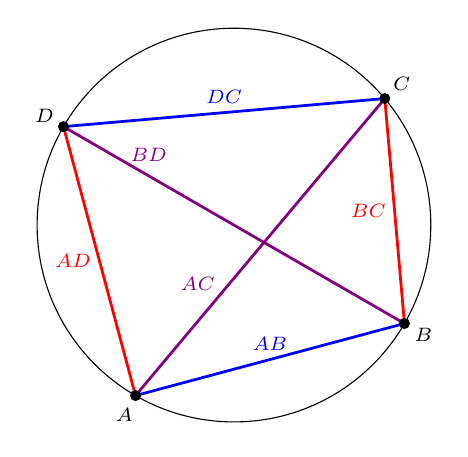
\begin{tikzpicture}
		\coordinate (center) at (0,0);
		\def\radius{2.5cm}
		\draw (center) circle[radius=\radius];

		% points on the circle
		\path (center) ++(-120:\radius) coordinate (A);
		\path (center) ++(-30:\radius) coordinate (B);
		\path (center) ++(40:\radius) coordinate (C);
		\path (center) ++(150:\radius) coordinate (D);

		\begin{scriptsize}
			% Chords
			\draw[color=red, line width=1pt] (A) -- node[left] {$AD$} (D);
			\draw[color=red, line width=1pt] (B) -- node[left] {$BC$} (C);
			\draw[color=blue, line width=1pt] (A) -- node[above] {$AB$} (B);
			\draw[color=blue, line width=1pt] (D) -- node[above] {$DC$} (C);
			\draw[color=violet, line width=1pt] (A) -- node[above=8pt, near start] {$AC$} (C);
			\draw[color=violet, line width=1pt] (D) -- node[above=2pt, near start] {$BD$} (B);

			% Draw the points over the chords
			\fill[black] (A) circle[radius=2pt] ++(-120:1em) node {$A$};
			\fill[black] (B) circle[radius=2pt] ++(-30:1em) node {$B$};
			\fill[black] (C) circle[radius=2pt] ++(40:1em) node {$C$};
			\fill[black] (D) circle[radius=2pt] ++(150:1em) node {$D$};

		\end{scriptsize}
	\end{tikzpicture}
	\caption{Ptolomy's theorem:
	${\color{violet} |AC| \cdot |BD|}
		= {\color{red} |AD|\cdot |BC|} + {\color{blue} |AB| \cdot |CD|}$.}
	\label{fig:ptolomy}
\end{figure}

Another thing we can notice, is that the relation resembles an exchange relation. We
will now use this intuition to place a cluster structure on $R_{2, m}$. Consider an
$m$-gon on a circle, with points labeled $1$ to $m$. A maximal triangularisation is a
maximal choice of pairwise non-crossing chords. Such a triangularisation will always
contain $m$ sides, and $m-3$ diagonals. Given a diagonal $d$, in such a maximal
triangularisation, it is the side of exactly two triangles, and hence a diagonal of the
quadrilateral formed by joining the two triangles. The \emph{flip} of this diagonal, is
then defined as replacing $d$ with the other diagonal of this quadrilateral. Applying
such flips yields new maximal triangularisations, and one can show that any maximal
triangularisation can be reached through a sequence of flips from any other
triangularisation.

Given a maximal triangularisation $\Delta$, we now define a quiver as follows (see
\cref{fig:triangularisation_quiver}):
\begin{itemize}
	\item The frozen vertices of the quiver are the sides of $\Delta$ (these are the same for any
	      triangularisation).
	\item The non-frozen vertices of the quiver are the diagonals of $\Delta$.
	\item Given two diagonals, or a diagonal and a side, sharing a vertex, we draw an edge
	      between them. For the orientation, consider the triangle containing these two chords.
	      The orientation is then taken such that the edges of the triangle are traversed in
	      clockwise order.
\end{itemize}

\begin{theorem}
	$R_{2,m}$ has a cluster structure of type $A_{m-3}$ such that:
	\begin{enumerate}
		\item Clusters are in one-to-one correspondence with the maximal triangularisations of the
		      $m$-gon.
		\item Mutations correspond to flipping.
		\item The chord $i \leftrightarrow j$ corresponds to $P_{ij}$.
		\item The exchange matrix is given by
		      \begin{equation*}
			      b_{ij}(\Delta) =
			      \begin{cases}
				      1  & \text{ if $i$ and $j$ are in a triangle and $j$ follows on $i$ } \\
				      -1 & \text{ if $i$ and $j$ are in a triangle and $i$ follows on $j$ } \\
				      0  & \text{ if $i$ and $j$ are not in a triangle}
			      \end{cases}
			      .
		      \end{equation*}
	\end{enumerate}
\end{theorem}

In \cref{fig:triangularisation_quiver} one can clearly see the path graph of $A_{m-3}$
appearing in the triangularisation on the right. It has actually also been shown that
$R_{k, m}$ has a cluster structure for $k > 2$, but the situation is a lot more
complex.

\begin{figure}

	\begin{center}
		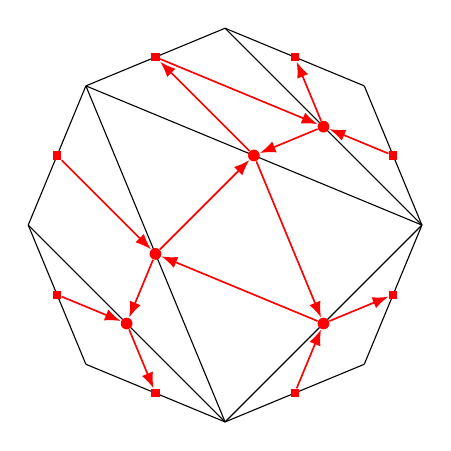
\begin{tikzpicture}
			\coordinate (center) at (0,0);
			\def\radius{2.5cm}

			% points on the circle
			\path (center) ++(0:\radius) coordinate (A);
			\path (center) ++(45:\radius) coordinate (B);
			\path (center) ++(90:\radius) coordinate (C);
			\path (center) ++(135:\radius) coordinate (D);
			\path (center) ++(180:\radius) coordinate (E);
			\path (center) ++(225:\radius) coordinate (F);
			\path (center) ++(270:\radius) coordinate (G);
			\path (center) ++(315:\radius) coordinate (H);

			% Sides with frozen verts
			\draw (A) -- node[rectangle, fill=red, inner sep=1.5pt] (AB) {} (B);
			\draw (B) -- node[rectangle, fill=red, inner sep=1.5pt] (BC) {} (C);
			\draw (C) -- node[rectangle, fill=red, inner sep=1.5pt] (CD) {} (D);
			\draw (D) -- node[rectangle, fill=red, inner sep=1.5pt] (DE) {} (E);
			\draw (E) -- node[rectangle, fill=red, inner sep=1.5pt] (EF) {} (F);
			\draw (F) -- node[rectangle, fill=red, inner sep=1.5pt] (FG) {} (G);
			\draw (G) -- node[rectangle, fill=red, inner sep=1.5pt] (GH) {} (H);
			\draw (H) -- node[rectangle, fill=red, inner sep=1.5pt] (HA) {} (A);

			% Diagonals with exchangeable verts
			\draw (A) -- node[circle, fill=red, inner sep=1.5pt] (AC) {} (C);
			\draw (A) -- node[circle, fill=red, inner sep=1.5pt] (AD) {} (D);
			\draw (A) -- node[circle, fill=red, inner sep=1.5pt] (AG) {} (G);
			\draw (D) -- node[circle, fill=red, inner sep=1.5pt] (DG) {} (G);
			\draw (E) -- node[circle, fill=red, inner sep=1.5pt] (EG) {} (G);

			% Quiver edges
			\draw[-Latex, red, line width=0.6pt] (AB) -- (AC);
			\draw[-Latex, red, line width=0.6pt] (AC) -- (BC);
			\draw[-Latex, red, line width=0.6pt] (AC) -- (AD);
			\draw[Latex-, red, line width=0.6pt] (AC) -- (CD);
			\draw[-Latex, red, line width=0.6pt] (AD) -- (CD);
			\draw[-Latex, red, line width=0.6pt] (AD) -- (AG);
			\draw[Latex-, red, line width=0.6pt] (AD) -- (DG);
			\draw[-Latex, red, line width=0.6pt] (AG) -- (DG);
			\draw[-Latex, red, line width=0.6pt] (AG) -- (HA);
			\draw[Latex-, red, line width=0.6pt] (AG) -- (GH);
			\draw[Latex-, red, line width=0.6pt] (DG) -- (DE);
			\draw[-Latex, red, line width=0.6pt] (DG) -- (EG);
			\draw[-Latex, red, line width=0.6pt] (EG) -- (FG);
			\draw[Latex-, red, line width=0.6pt] (EG) -- (EF);

		\end{tikzpicture}
		\hspace{1cm}
		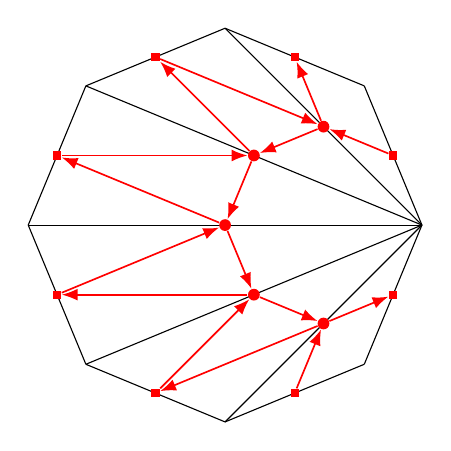
\begin{tikzpicture}
			\coordinate (center) at (0,0);
			\def\radius{2.5cm}

			% points on the circle
			\path (center) ++(0:\radius) coordinate (A);
			\path (center) ++(45:\radius) coordinate (B);
			\path (center) ++(90:\radius) coordinate (C);
			\path (center) ++(135:\radius) coordinate (D);
			\path (center) ++(180:\radius) coordinate (E);
			\path (center) ++(225:\radius) coordinate (F);
			\path (center) ++(270:\radius) coordinate (G);
			\path (center) ++(315:\radius) coordinate (H);

			% Sides with frozen verts
			\draw (A) -- node[rectangle, fill=red, inner sep=1.5pt] (AB) {} (B);
			\draw (B) -- node[rectangle, fill=red, inner sep=1.5pt] (BC) {} (C);
			\draw (C) -- node[rectangle, fill=red, inner sep=1.5pt] (CD) {} (D);
			\draw (D) -- node[rectangle, fill=red, inner sep=1.5pt] (DE) {} (E);
			\draw (E) -- node[rectangle, fill=red, inner sep=1.5pt] (EF) {} (F);
			\draw (F) -- node[rectangle, fill=red, inner sep=1.5pt] (FG) {} (G);
			\draw (G) -- node[rectangle, fill=red, inner sep=1.5pt] (GH) {} (H);
			\draw (H) -- node[rectangle, fill=red, inner sep=1.5pt] (HA) {} (A);

			% Diagonals with exchangeable verts
			\draw (A) -- node[circle, fill=red, inner sep=1.5pt] (AC) {} (C);
			\draw (A) -- node[circle, fill=red, inner sep=1.5pt] (AD) {} (D);
			\draw (A) -- node[circle, fill=red, inner sep=1.5pt] (AE) {} (E);
			\draw (A) -- node[circle, fill=red, inner sep=1.5pt] (AF) {} (F);
			\draw (A) -- node[circle, fill=red, inner sep=1.5pt] (AG) {} (G);

			% Quiver edges between exchangeable
			\draw[-Latex, red, line width=0.6pt] (AC) -- (AD);
			\draw[-Latex, red, line width=0.6pt] (AD) -- (AE);
			\draw[-Latex, red, line width=0.6pt] (AE) -- (AF);
			\draw[-Latex, red, line width=0.6pt] (AF) -- (AG);
			\draw[-Latex, red, line width=0.6pt] (AG) -- (HA);

			% Quiver edges with frozen vertices

			\draw[-Latex, red, line width=0.6pt] (AB) -- (AC);
			\draw[-Latex, red, line width=0.6pt] (AC) -- (BC);
			\draw[Latex-, red, line width=0.6pt] (AC) -- (CD);
			\draw[-Latex, red, line width=0.6pt] (AD) -- (CD);
			\draw[Latex-, red, line width=0.6pt] (AD) -- (DE);
			\draw[-Latex, red, line width=0.6pt] (AE) -- (DE);
			\draw[Latex-, red, line width=0.6pt] (AE) -- (EF);
			\draw[-Latex, red, line width=0.6pt] (AF) -- (EF);
			\draw[Latex-, red, line width=0.6pt] (AF) -- (FG);
			\draw[-Latex, red, line width=0.6pt] (AG) -- (FG);
			\draw[Latex-, red, line width=0.6pt] (AG) -- (GH);

		\end{tikzpicture}
	\end{center}

	\caption{The quiver associated to a triangularisation.}
	\label{fig:triangularisation_quiver}
\end{figure}

\bibliographystyle{plain}
\bibliography{references.bib}

\end{document}